% Options for packages loaded elsewhere
\PassOptionsToPackage{unicode}{hyperref}
\PassOptionsToPackage{hyphens}{url}
%
\documentclass[
]{article}
\usepackage{lmodern}
\usepackage{amssymb,amsmath}
\usepackage{ifxetex,ifluatex}
\ifnum 0\ifxetex 1\fi\ifluatex 1\fi=0 % if pdftex
  \usepackage[T1]{fontenc}
  \usepackage[utf8]{inputenc}
  \usepackage{textcomp} % provide euro and other symbols
\else % if luatex or xetex
  \usepackage{unicode-math}
  \defaultfontfeatures{Scale=MatchLowercase}
  \defaultfontfeatures[\rmfamily]{Ligatures=TeX,Scale=1}
\fi
% Use upquote if available, for straight quotes in verbatim environments
\IfFileExists{upquote.sty}{\usepackage{upquote}}{}
\IfFileExists{microtype.sty}{% use microtype if available
  \usepackage[]{microtype}
  \UseMicrotypeSet[protrusion]{basicmath} % disable protrusion for tt fonts
}{}
\makeatletter
\@ifundefined{KOMAClassName}{% if non-KOMA class
  \IfFileExists{parskip.sty}{%
    \usepackage{parskip}
  }{% else
    \setlength{\parindent}{0pt}
    \setlength{\parskip}{6pt plus 2pt minus 1pt}}
}{% if KOMA class
  \KOMAoptions{parskip=half}}
\makeatother
\usepackage{xcolor}
\IfFileExists{xurl.sty}{\usepackage{xurl}}{} % add URL line breaks if available
\IfFileExists{bookmark.sty}{\usepackage{bookmark}}{\usepackage{hyperref}}
\hypersetup{
  pdftitle={Patterns of performance degradation during sleep restriction of long distance truck drivers},
  pdfauthor={Laura Bogeart, Ben De Maesschalck, Bianca Florenzi, Jonas Jonker, Nina Rank, Alexandra Stanciu, Maria Tsontaki, Dries Vrijens},
  hidelinks,
  pdfcreator={LaTeX via pandoc}}
\urlstyle{same} % disable monospaced font for URLs
\usepackage[margin=1in]{geometry}
\usepackage{longtable,booktabs}
% Correct order of tables after \paragraph or \subparagraph
\usepackage{etoolbox}
\makeatletter
\patchcmd\longtable{\par}{\if@noskipsec\mbox{}\fi\par}{}{}
\makeatother
% Allow footnotes in longtable head/foot
\IfFileExists{footnotehyper.sty}{\usepackage{footnotehyper}}{\usepackage{footnote}}
\makesavenoteenv{longtable}
\usepackage{graphicx}
\makeatletter
\def\maxwidth{\ifdim\Gin@nat@width>\linewidth\linewidth\else\Gin@nat@width\fi}
\def\maxheight{\ifdim\Gin@nat@height>\textheight\textheight\else\Gin@nat@height\fi}
\makeatother
% Scale images if necessary, so that they will not overflow the page
% margins by default, and it is still possible to overwrite the defaults
% using explicit options in \includegraphics[width, height, ...]{}
\setkeys{Gin}{width=\maxwidth,height=\maxheight,keepaspectratio}
% Set default figure placement to htbp
\makeatletter
\def\fps@figure{htbp}
\makeatother
\setlength{\emergencystretch}{3em} % prevent overfull lines
\providecommand{\tightlist}{%
  \setlength{\itemsep}{0pt}\setlength{\parskip}{0pt}}
\setcounter{secnumdepth}{-\maxdimen} % remove section numbering
% https://github.com/rstudio/rmarkdown/issues/337
\let\rmarkdownfootnote\footnote%
\def\footnote{\protect\rmarkdownfootnote}

% https://github.com/rstudio/rmarkdown/pull/252
\usepackage{titling}
\setlength{\droptitle}{-2em}

\pretitle{\vspace{\droptitle}\centering\huge}
\posttitle{\par}

\preauthor{\centering\large\emph}
\postauthor{\par}

\predate{\centering\large\emph}
\postdate{\par}

\title{Patterns of performance degradation during sleep restriction of
long distance truck drivers}
\author{Laura Bogeart, Ben De Maesschalck, Bianca Florenzi, Jonas
Jonker, Nina Rank, Alexandra Stanciu, Maria Tsontaki, Dries Vrijens}
\date{}

\begin{document}
\maketitle

\hypertarget{presentation-of-the-case-study}{%
\subsection{Presentation of the case
study}\label{presentation-of-the-case-study}}

We are analysing the effect of sleep deprivation on reaction time of
long distance truck drivers. There are 18 subjects in the dataset and
for each subject, the reaction time was measured for 10 days. The
subjects were allowed only a limited amount of sleep for these 10
subsequent days. Each subject's reaction time was measured several times
on each day of the trial and an average was taken. Reaction time is
measured with a psychomotor vigilance task (PVT), which measures the
speed with which subjects respond to a visual stimulus.

Our research questions is: Is there any relation between reaction time
and the number of days of sleep deprivation?

\hypertarget{exploratory-analysis}{%
\subsection{Exploratory analysis}\label{exploratory-analysis}}

\begin{longtable}[]{@{}ccc@{}}
\toprule
\begin{minipage}[b]{0.14\columnwidth}\centering
Reaction\strut
\end{minipage} & \begin{minipage}[b]{0.09\columnwidth}\centering
Days\strut
\end{minipage} & \begin{minipage}[b]{0.13\columnwidth}\centering
Subject\strut
\end{minipage}\tabularnewline
\midrule
\endhead
\begin{minipage}[t]{0.14\columnwidth}\centering
249.6\strut
\end{minipage} & \begin{minipage}[t]{0.09\columnwidth}\centering
0\strut
\end{minipage} & \begin{minipage}[t]{0.13\columnwidth}\centering
308\strut
\end{minipage}\tabularnewline
\begin{minipage}[t]{0.14\columnwidth}\centering
258.7\strut
\end{minipage} & \begin{minipage}[t]{0.09\columnwidth}\centering
1\strut
\end{minipage} & \begin{minipage}[t]{0.13\columnwidth}\centering
308\strut
\end{minipage}\tabularnewline
\begin{minipage}[t]{0.14\columnwidth}\centering
250.8\strut
\end{minipage} & \begin{minipage}[t]{0.09\columnwidth}\centering
2\strut
\end{minipage} & \begin{minipage}[t]{0.13\columnwidth}\centering
308\strut
\end{minipage}\tabularnewline
\begin{minipage}[t]{0.14\columnwidth}\centering
321.4\strut
\end{minipage} & \begin{minipage}[t]{0.09\columnwidth}\centering
3\strut
\end{minipage} & \begin{minipage}[t]{0.13\columnwidth}\centering
308\strut
\end{minipage}\tabularnewline
\begin{minipage}[t]{0.14\columnwidth}\centering
356.9\strut
\end{minipage} & \begin{minipage}[t]{0.09\columnwidth}\centering
4\strut
\end{minipage} & \begin{minipage}[t]{0.13\columnwidth}\centering
308\strut
\end{minipage}\tabularnewline
\begin{minipage}[t]{0.14\columnwidth}\centering
414.7\strut
\end{minipage} & \begin{minipage}[t]{0.09\columnwidth}\centering
5\strut
\end{minipage} & \begin{minipage}[t]{0.13\columnwidth}\centering
308\strut
\end{minipage}\tabularnewline
\begin{minipage}[t]{0.14\columnwidth}\centering
382.2\strut
\end{minipage} & \begin{minipage}[t]{0.09\columnwidth}\centering
6\strut
\end{minipage} & \begin{minipage}[t]{0.13\columnwidth}\centering
308\strut
\end{minipage}\tabularnewline
\begin{minipage}[t]{0.14\columnwidth}\centering
290.1\strut
\end{minipage} & \begin{minipage}[t]{0.09\columnwidth}\centering
7\strut
\end{minipage} & \begin{minipage}[t]{0.13\columnwidth}\centering
308\strut
\end{minipage}\tabularnewline
\begin{minipage}[t]{0.14\columnwidth}\centering
430.6\strut
\end{minipage} & \begin{minipage}[t]{0.09\columnwidth}\centering
8\strut
\end{minipage} & \begin{minipage}[t]{0.13\columnwidth}\centering
308\strut
\end{minipage}\tabularnewline
\begin{minipage}[t]{0.14\columnwidth}\centering
466.4\strut
\end{minipage} & \begin{minipage}[t]{0.09\columnwidth}\centering
9\strut
\end{minipage} & \begin{minipage}[t]{0.13\columnwidth}\centering
308\strut
\end{minipage}\tabularnewline
\bottomrule
\end{longtable}

This dataset contains multiple measurements for each subject on
consecutive days, with as response variable the continuous variable
reaction time and explanatory variable days. Since there are 10
measurements for each subject, it is a longitudinal study. The dataset
of 18 subjects is balanced and complete with an equal amount of
measurements for each subject (i.e.~no missing data).

\hypertarget{spaghetti-plot}{%
\subsubsection{Spaghetti Plot}\label{spaghetti-plot}}

To visualise the individual reaction times and how they compare to the
mean, a spaghetti plot was created. This revealed that there was
variation in intercepts or starting reaction times on day 0 between
subjects. This variation between subjects increased with subsequent
days.

For most subjects, the reaction time increased with the amount of days
of sleep deprivation. This increase is also visible in the mean.

\begin{center}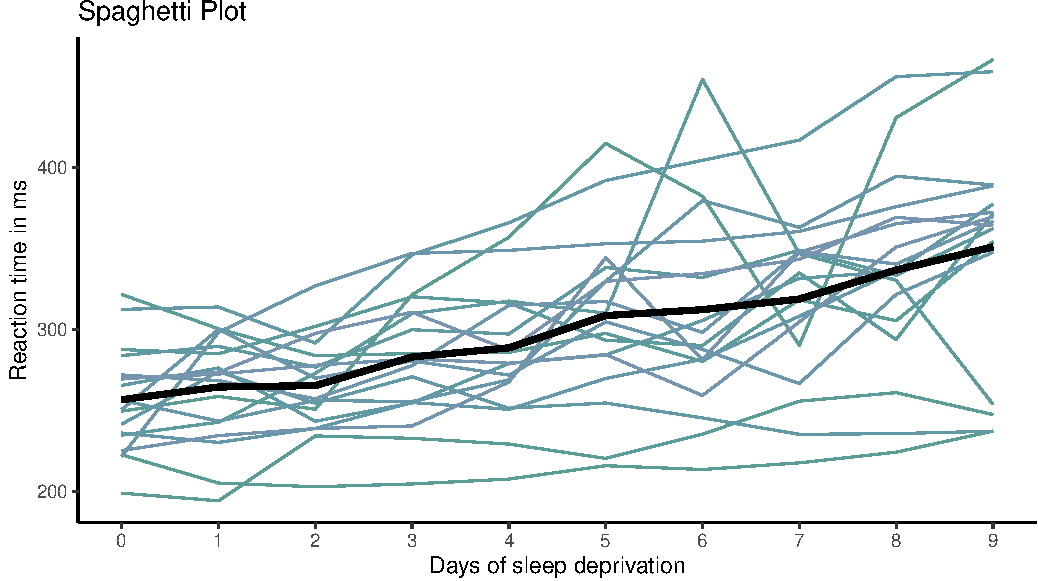
\includegraphics{common_sleep_files/figure-latex/spaghetti-1} \end{center}

\hypertarget{boxplot-violin-plot-and-mean-evolution}{%
\subsection{Boxplot, Violin plot and Mean
evolution}\label{boxplot-violin-plot-and-mean-evolution}}

The following boxplot (A) was created to get a quick summary of the
dataset's characteristics. The mean and median seem to show a similar
increase throughout the study. For day nr 5, 6 and 9, outliers are
observed. We observe that the variance increases with an increase in
days of sleep deprivation but the interquartile range appears to expand
not as strongly as the minimum and maximum of the boxplot.

To put together, some subjects deviate more from the mean with an
increase in days of sleep deprivation (see outliers on both sides) while
most others stay around the mean (see slower increase in interquartile
range).

The violin plot (B) supports the above observations of the distribution
of the data around the mean with outliers.

To further support our previous findings, we looked at the mean
evolution (C). Here, a trend of increasing reaction time with increasing
number of days is also observed, together with an expanding standard
deviation (see errorbars).

\begin{center}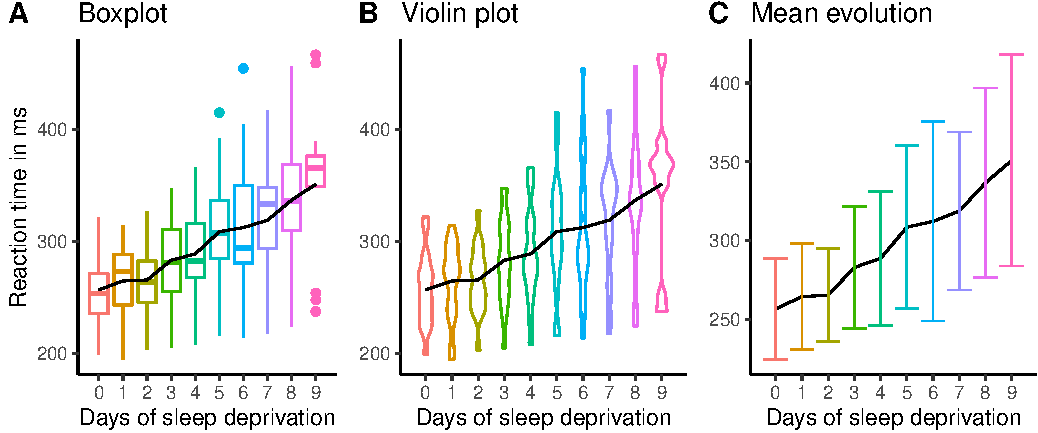
\includegraphics{common_sleep_files/figure-latex/boxplot-1} \end{center}

\hypertarget{descriptives}{%
\subsection{Descriptives}\label{descriptives}}

\begin{longtable}[]{@{}lrrrrr@{}}
\toprule
& Days & Mean & SD & Var & n\tabularnewline
\midrule
\endhead
0 & 0 & 256.65 & 32.13 & 1032.30 & 18\tabularnewline
1 & 1 & 264.50 & 33.43 & 1117.59 & 18\tabularnewline
2 & 2 & 265.36 & 29.47 & 868.68 & 18\tabularnewline
3 & 3 & 282.99 & 38.86 & 1509.92 & 18\tabularnewline
4 & 4 & 288.65 & 42.54 & 1809.47 & 18\tabularnewline
5 & 5 & 308.52 & 51.77 & 2680.09 & 18\tabularnewline
6 & 6 & 312.18 & 63.17 & 3990.92 & 18\tabularnewline
7 & 7 & 318.75 & 50.10 & 2510.41 & 18\tabularnewline
8 & 8 & 336.63 & 60.20 & 3624.01 & 18\tabularnewline
9 & 9 & 350.85 & 66.99 & 4487.15 & 18\tabularnewline
\bottomrule
\end{longtable}

The calculations of the mean, standard deviation and variance of the
reaction time for each day of all subjects further support our
exploratory plots: we observe an overall increase in the mean, variance
and standard deviation with more days of sleep deprivation. (Note that
for day 2 and 7 the variance and standard deviation decrease compared to
the previous day. It continues to increase afterwards, however).

\hypertarget{correlation}{%
\subsection{Correlation}\label{correlation}}

\begin{center}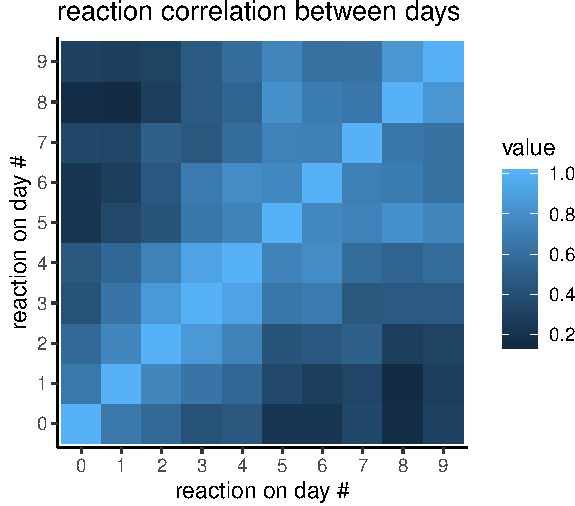
\includegraphics{common_sleep_files/figure-latex/spearman_tile-1} \end{center}

We used the Shapiro - Wilk test to check for the normality of the
reaction times per day. The test revealed a non normal distribution of
day 9. Thus, we performed the spearman correlation method instead of
pearson to check for a correlation of the reaction times between days.

Looking at the correlation matrix, there is a correlation higher than
0.6 between subsequent days (e.g.~between Day 3 and 4, between Day 8 and
9, etc). However, the further the days are apart, the lower the
correlation (e.g.~low correlation between Day 1 and Day 8).

\hypertarget{regression-per-person}{%
\subsection{Regression per person}\label{regression-per-person}}

\begin{center}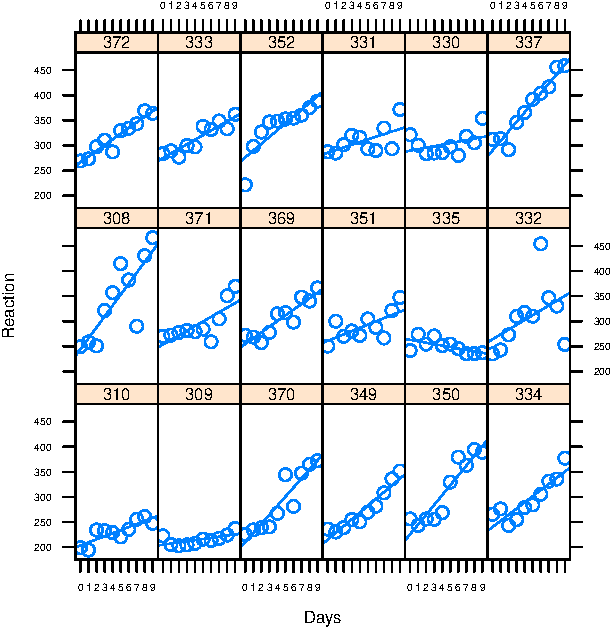
\includegraphics{common_sleep_files/figure-latex/trellis-1} \end{center}

We performed a linear regression model on each subject based on the
function: \[\text{reaction time (Reaction)} = b_0 + b_i* \text{Days}\]

We then created a trellis graph to visualise the intercepts and slopes
of these subject-specific linear regression models.

The graph suggests that the slope and intercept of each subject's linear
model are independent of each other as there is no observable trend
between the height of the intercept and the steepness of the slope. This
is further supported by plotting the intercept against the slope (see
chapter ``OLS vs.~LMM'', Fig. A (orange dots)). Overall, all subjects
have a positive slope besides subject 335.

The linear regression lines fit the datapoints closely, suggesting that
a linear model is appropriate to represent this dataset.

\hypertarget{between-subject-variability}{%
\subsection{Between subject
variability}\label{between-subject-variability}}

\begin{center}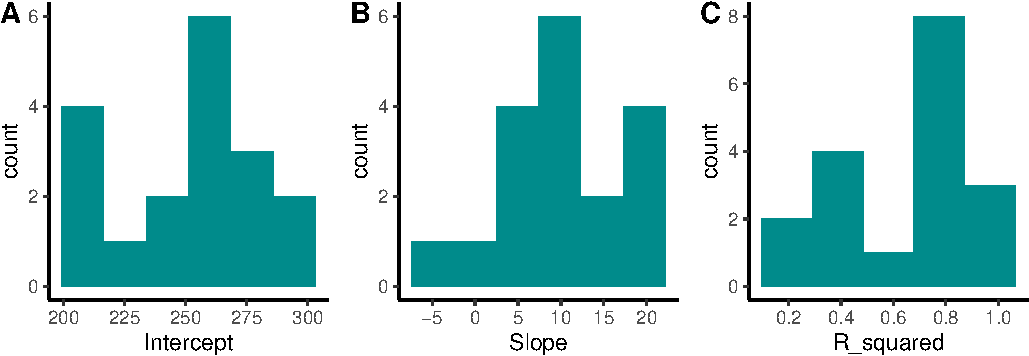
\includegraphics{common_sleep_files/figure-latex/unnamed-chunk-3-1} \end{center}

The individual intercepts shown in the first histogram (A) correspond to
the initial reaction time at day zero and are non normally distributed.
Given the small data set, this is not surprising as it shows a variety
of the initial reaction time. However, if this data came from a large
dataset, it would be surprising that the initial data points are not
normally distributed and could suggest a wrong data sample compared to
the population.

Looking at the histogram of individual slopes (B), we see a normal
distribution. As seen on the previous graph showcasing the individual
linear regressions, only one slope is negative. This shows again that
reaction time increases by days of sleep deprivation.

Finally, looking at the histogram of R squared (C), we see that the
majority of subjects have a R squared of above 0.6. This shows that the
linear model is appropriate for this data set. However, the individual
linear model does not fit the specific data of some subjects,
respectively 7 of the 18 subjects.

\hypertarget{fitting-the-model---with-reml}{%
\subsection{Fitting the model - with
REML}\label{fitting-the-model---with-reml}}

\hypertarget{mathematical-description}{%
\subsection{Mathematical description}\label{mathematical-description}}

Level 1 model explains the evolution of Reaction time for each subject:
\[\begin{aligned}
Y_{ij}&= \pi_{0i} + \pi_{1i}* \text{Days}_{ij} && \text{how do individuals evolve} \\
          &+ \epsilon_{ij} &&\text{how the individuals deviate from their own evolution}
\end{aligned}\]

Level 2 model explains why the Subjects differ from each other:
\[\begin{aligned}
\pi_{0i} &= \gamma_{0} + b_{0i} && \text{explains the intercept} \\
\pi_{1i} &= \gamma_{1} + b_{1i} && \text{explains the slope}
\end{aligned}\]

\(\sigma_{0}^{2}\) - Level 2 residual variance in true intercept
\(\pi_{0i}\) across all individuals in the population

\(\sigma_{1}^{2}\) - Level 2 residual variance in true slope
\(\pi_{1i}\) across all individuals in the population

With the level 2 model we are trying to explain the variation between
individuals using the intercept and at the slope while \(b_{0i}\) and
\(b_{1i}\) describe the unexplained variability between subjects.

The full model describes the evolution observed in the spaghetti plot
and other descriptive plots of the data: \[\begin{aligned}
Y_{ij} =& \gamma_{0} + \gamma_{1}* \text{Days}_{ij} &&\text{fixed effects}\\
          &+ b_{0i} + b_{1i}*\text{Days}_{ij} &&\text{random effect}\\
          &+ \epsilon_{ij} &&\text{error}
\end{aligned}\]

\[
\begin{cases}
Y_{ij} &= \pi_{0i} + \pi_{1i}* \text{Days}_{ij} + \epsilon_{ij} \\
\pi_{0i} &= \gamma_{0} + b_{0i}  \\
\pi_{1i} &= \gamma_{1} + b_{1i}
\end{cases}
\]

Underneath is the average evolution of the whole population:
\[E(Y_{ij}) = \gamma_{0} + \gamma_{1}* \text{Days}_{ij}\]

The general linear mixed model is given by: \[\begin{cases}
Y_i = X_i\beta + Z_i b_i + \epsilon_i \\
b_i \sim N(0,D)\\
\epsilon_i \sim N(0,\Sigma_i)
\end{cases}\]

\[Y_i \sim N(X_i\beta, Z_iDZ_i'+\Sigma_i)\]

R uses the marginal model and our calcuation are based on that.

\begin{verbatim}
## Linear mixed model fit by REML ['lmerMod']
## Formula: Reaction ~ 1 + Days + (1 + Days | Subject)
##    Data: sleep
## 
## REML criterion at convergence: 1743.6
## 
## Scaled residuals: 
##     Min      1Q  Median      3Q     Max 
## -3.9536 -0.4634  0.0231  0.4633  5.1793 
## 
## Random effects:
##  Groups   Name        Variance Std.Dev. Corr
##  Subject  (Intercept) 611.90   24.737       
##           Days         35.08    5.923   0.07
##  Residual             654.94   25.592       
## Number of obs: 180, groups:  Subject, 18
## 
## Fixed effects:
##             Estimate Std. Error t value
## (Intercept)  251.405      6.824  36.843
## Days          10.467      1.546   6.771
## 
## Correlation of Fixed Effects:
##      (Intr)
## Days -0.138
\end{verbatim}

\hypertarget{values-of-the-reml-model}{%
\subsection{Values of the REML model}\label{values-of-the-reml-model}}

Based on the above model, we find the following values:

\[\begin{aligned}
\gamma_{0}  &= 251.405 \\
\gamma_{1}  &= 10.467  \\
\sigma_{\epsilon}^{2} &= 654.94 \\
\sigma_{0}^{2} &= 611.90 \\
\sigma_{1}^{2} &= 35.08 \\
corr(b_{0i}, b_{1i}) &= 0.07
\end{aligned}\]

\[
\begin{cases}
Y_{ij}   &= \pi_{0i} + \pi_{1i}* Days_{ij} + \epsilon_{ij} \\
\pi_{0i} &= 251.41 + b_{0i} \\
\pi_{1i} &= 10.47 + b_{1i}
\end{cases}
\]

\[\epsilon_{ij} \sim N(0,25.59^2)\]

\[
\begin{pmatrix} b_{0i} \\ b_{1i} \end{pmatrix}
\sim N
\begin{pmatrix}
\begin{pmatrix} 0 \\ 0 \end{pmatrix},
\begin{pmatrix}
\sigma_{0}^2 & \sigma_{01} \\
\sigma_{01} & \sigma_{1}^2 
\end{pmatrix}
\end{pmatrix}
\] \[
\begin{pmatrix} b_{0i} \\ b_{1i} \end{pmatrix}
\sim N
\begin{pmatrix}
\begin{pmatrix} 0 \\ 0 \end{pmatrix},
\begin{pmatrix}
611.9 & 9.61 \\
9.61 & 35.08 
\end{pmatrix}
\end{pmatrix}
\]

Next step is to check if the values retrieved are actually significant.
We therefore check if the number of days have a significant effect on
the reaction time.

In the next chapter, we tested the fixed effects with Bootstrap and
profile likelihood as the sample size was too small to use a Wald test.
Next, we checked and compared different possible models using a
likelihood ratio test.

\hypertarget{testing-fixed-effects---with-bootstrap}{%
\subsection{Testing fixed effects - with
bootstrap}\label{testing-fixed-effects---with-bootstrap}}

Computing bootstrap confidence intervals \ldots{}

6 message(s): boundary (singular) fit: see ?isSingular 147 warning(s):
Model failed to converge with max\textbar grad\textbar{} = 0.00200417
(tol = 0.002, component 1) (and others)

\begin{longtable}[]{@{}ccc@{}}
\toprule
\begin{minipage}[b]{0.44\columnwidth}\centering
~\strut
\end{minipage} & \begin{minipage}[b]{0.13\columnwidth}\centering
2.5 \%\strut
\end{minipage} & \begin{minipage}[b]{0.13\columnwidth}\centering
97.5 \%\strut
\end{minipage}\tabularnewline
\midrule
\endhead
\begin{minipage}[t]{0.44\columnwidth}\centering
\textbf{sd\_(Intercept)\textbar Subject}\strut
\end{minipage} & \begin{minipage}[t]{0.13\columnwidth}\centering
11.76\strut
\end{minipage} & \begin{minipage}[t]{0.13\columnwidth}\centering
34.95\strut
\end{minipage}\tabularnewline
\begin{minipage}[t]{0.44\columnwidth}\centering
\textbf{cor\_Days.(Intercept)\textbar Subject}\strut
\end{minipage} & \begin{minipage}[t]{0.13\columnwidth}\centering
-0.4596\strut
\end{minipage} & \begin{minipage}[t]{0.13\columnwidth}\centering
0.8595\strut
\end{minipage}\tabularnewline
\begin{minipage}[t]{0.44\columnwidth}\centering
\textbf{sd\_Days\textbar Subject}\strut
\end{minipage} & \begin{minipage}[t]{0.13\columnwidth}\centering
3.415\strut
\end{minipage} & \begin{minipage}[t]{0.13\columnwidth}\centering
8.295\strut
\end{minipage}\tabularnewline
\begin{minipage}[t]{0.44\columnwidth}\centering
\textbf{sigma}\strut
\end{minipage} & \begin{minipage}[t]{0.13\columnwidth}\centering
22.5\strut
\end{minipage} & \begin{minipage}[t]{0.13\columnwidth}\centering
28.56\strut
\end{minipage}\tabularnewline
\begin{minipage}[t]{0.44\columnwidth}\centering
\textbf{(Intercept)}\strut
\end{minipage} & \begin{minipage}[t]{0.13\columnwidth}\centering
237.7\strut
\end{minipage} & \begin{minipage}[t]{0.13\columnwidth}\centering
265.3\strut
\end{minipage}\tabularnewline
\begin{minipage}[t]{0.44\columnwidth}\centering
\textbf{Days}\strut
\end{minipage} & \begin{minipage}[t]{0.13\columnwidth}\centering
7.681\strut
\end{minipage} & \begin{minipage}[t]{0.13\columnwidth}\centering
13.62\strut
\end{minipage}\tabularnewline
\bottomrule
\end{longtable}

Computing profile confidence intervals \ldots{}

\begin{longtable}[]{@{}ccc@{}}
\toprule
\begin{minipage}[b]{0.44\columnwidth}\centering
~\strut
\end{minipage} & \begin{minipage}[b]{0.13\columnwidth}\centering
2.5 \%\strut
\end{minipage} & \begin{minipage}[b]{0.13\columnwidth}\centering
97.5 \%\strut
\end{minipage}\tabularnewline
\midrule
\endhead
\begin{minipage}[t]{0.44\columnwidth}\centering
\textbf{sd\_(Intercept)\textbar Subject}\strut
\end{minipage} & \begin{minipage}[t]{0.13\columnwidth}\centering
14.38\strut
\end{minipage} & \begin{minipage}[t]{0.13\columnwidth}\centering
37.72\strut
\end{minipage}\tabularnewline
\begin{minipage}[t]{0.44\columnwidth}\centering
\textbf{cor\_Days.(Intercept)\textbar Subject}\strut
\end{minipage} & \begin{minipage}[t]{0.13\columnwidth}\centering
-0.4815\strut
\end{minipage} & \begin{minipage}[t]{0.13\columnwidth}\centering
0.685\strut
\end{minipage}\tabularnewline
\begin{minipage}[t]{0.44\columnwidth}\centering
\textbf{sd\_Days\textbar Subject}\strut
\end{minipage} & \begin{minipage}[t]{0.13\columnwidth}\centering
3.801\strut
\end{minipage} & \begin{minipage}[t]{0.13\columnwidth}\centering
8.753\strut
\end{minipage}\tabularnewline
\begin{minipage}[t]{0.44\columnwidth}\centering
\textbf{sigma}\strut
\end{minipage} & \begin{minipage}[t]{0.13\columnwidth}\centering
22.9\strut
\end{minipage} & \begin{minipage}[t]{0.13\columnwidth}\centering
28.86\strut
\end{minipage}\tabularnewline
\begin{minipage}[t]{0.44\columnwidth}\centering
\textbf{(Intercept)}\strut
\end{minipage} & \begin{minipage}[t]{0.13\columnwidth}\centering
237.7\strut
\end{minipage} & \begin{minipage}[t]{0.13\columnwidth}\centering
265.1\strut
\end{minipage}\tabularnewline
\begin{minipage}[t]{0.44\columnwidth}\centering
\textbf{Days}\strut
\end{minipage} & \begin{minipage}[t]{0.13\columnwidth}\centering
7.359\strut
\end{minipage} & \begin{minipage}[t]{0.13\columnwidth}\centering
13.58\strut
\end{minipage}\tabularnewline
\bottomrule
\end{longtable}

The confidence intervals of the intercept and Days do not include 0.
Therefore, both have a significant effect on the Reaction time.

\hypertarget{likelihood-ratio-test-with-anova}{%
\subsection{Likelihood ratio test with
Anova}\label{likelihood-ratio-test-with-anova}}

\begin{longtable}[]{@{}cccccccc@{}}
\caption{Data: sleep (continued below)}\tabularnewline
\toprule
\begin{minipage}[b]{0.22\columnwidth}\centering
~\strut
\end{minipage} & \begin{minipage}[b]{0.05\columnwidth}\centering
Df\strut
\end{minipage} & \begin{minipage}[b]{0.07\columnwidth}\centering
AIC\strut
\end{minipage} & \begin{minipage}[b]{0.07\columnwidth}\centering
BIC\strut
\end{minipage} & \begin{minipage}[b]{0.09\columnwidth}\centering
logLik\strut
\end{minipage} & \begin{minipage}[b]{0.11\columnwidth}\centering
deviance\strut
\end{minipage} & \begin{minipage}[b]{0.08\columnwidth}\centering
Chisq\strut
\end{minipage} & \begin{minipage}[b]{0.09\columnwidth}\centering
Chi Df\strut
\end{minipage}\tabularnewline
\midrule
\endfirsthead
\toprule
\begin{minipage}[b]{0.22\columnwidth}\centering
~\strut
\end{minipage} & \begin{minipage}[b]{0.05\columnwidth}\centering
Df\strut
\end{minipage} & \begin{minipage}[b]{0.07\columnwidth}\centering
AIC\strut
\end{minipage} & \begin{minipage}[b]{0.07\columnwidth}\centering
BIC\strut
\end{minipage} & \begin{minipage}[b]{0.09\columnwidth}\centering
logLik\strut
\end{minipage} & \begin{minipage}[b]{0.11\columnwidth}\centering
deviance\strut
\end{minipage} & \begin{minipage}[b]{0.08\columnwidth}\centering
Chisq\strut
\end{minipage} & \begin{minipage}[b]{0.09\columnwidth}\centering
Chi Df\strut
\end{minipage}\tabularnewline
\midrule
\endhead
\begin{minipage}[t]{0.22\columnwidth}\centering
\textbf{sleep.intercept}\strut
\end{minipage} & \begin{minipage}[t]{0.05\columnwidth}\centering
3\strut
\end{minipage} & \begin{minipage}[t]{0.07\columnwidth}\centering
1917\strut
\end{minipage} & \begin{minipage}[t]{0.07\columnwidth}\centering
1926\strut
\end{minipage} & \begin{minipage}[t]{0.09\columnwidth}\centering
-955.3\strut
\end{minipage} & \begin{minipage}[t]{0.11\columnwidth}\centering
1911\strut
\end{minipage} & \begin{minipage}[t]{0.08\columnwidth}\centering
NA\strut
\end{minipage} & \begin{minipage}[t]{0.09\columnwidth}\centering
NA\strut
\end{minipage}\tabularnewline
\begin{minipage}[t]{0.22\columnwidth}\centering
\textbf{sleep.full}\strut
\end{minipage} & \begin{minipage}[t]{0.05\columnwidth}\centering
6\strut
\end{minipage} & \begin{minipage}[t]{0.07\columnwidth}\centering
1764\strut
\end{minipage} & \begin{minipage}[t]{0.07\columnwidth}\centering
1783\strut
\end{minipage} & \begin{minipage}[t]{0.09\columnwidth}\centering
-876\strut
\end{minipage} & \begin{minipage}[t]{0.11\columnwidth}\centering
1752\strut
\end{minipage} & \begin{minipage}[t]{0.08\columnwidth}\centering
158.6\strut
\end{minipage} & \begin{minipage}[t]{0.09\columnwidth}\centering
3\strut
\end{minipage}\tabularnewline
\bottomrule
\end{longtable}

\begin{longtable}[]{@{}cc@{}}
\toprule
\begin{minipage}[b]{0.29\columnwidth}\centering
~\strut
\end{minipage} & \begin{minipage}[b]{0.17\columnwidth}\centering
Pr(\textgreater Chisq)\strut
\end{minipage}\tabularnewline
\midrule
\endhead
\begin{minipage}[t]{0.29\columnwidth}\centering
\textbf{sleep.intercept}\strut
\end{minipage} & \begin{minipage}[t]{0.17\columnwidth}\centering
NA\strut
\end{minipage}\tabularnewline
\begin{minipage}[t]{0.29\columnwidth}\centering
\textbf{sleep.full}\strut
\end{minipage} & \begin{minipage}[t]{0.17\columnwidth}\centering
3.672e-34\strut
\end{minipage}\tabularnewline
\bottomrule
\end{longtable}

We compared an intercept-only model with a model that includes Days to
find the best model using MLE.

Looking at the outcome of the likelihood ratio test with Anova, we can
conclude that adding Days as covariate improves our model significantly.
Days has a significant effect on the Reaction time with a p-value much
smaller than 0.05.

The decrease in AIC value also supports this conclusion.

\hypertarget{testing-the-random-effects}{%
\subsection{Testing the random
effects}\label{testing-the-random-effects}}

\begin{longtable}[]{@{}ccc@{}}
\toprule
\begin{minipage}[b]{0.23\columnwidth}\centering
~\strut
\end{minipage} & \begin{minipage}[b]{0.18\columnwidth}\centering
(Intercept)\strut
\end{minipage} & \begin{minipage}[b]{0.10\columnwidth}\centering
Days\strut
\end{minipage}\tabularnewline
\midrule
\endhead
\begin{minipage}[t]{0.23\columnwidth}\centering
\textbf{(Intercept)}\strut
\end{minipage} & \begin{minipage}[t]{0.18\columnwidth}\centering
611.9\strut
\end{minipage} & \begin{minipage}[t]{0.10\columnwidth}\centering
9.614\strut
\end{minipage}\tabularnewline
\begin{minipage}[t]{0.23\columnwidth}\centering
\textbf{Days}\strut
\end{minipage} & \begin{minipage}[t]{0.18\columnwidth}\centering
9.614\strut
\end{minipage} & \begin{minipage}[t]{0.10\columnwidth}\centering
35.08\strut
\end{minipage}\tabularnewline
\bottomrule
\end{longtable}

Firstly, we check the random effects covariance matrix.

The model is built on the assumption that the b's come from a normal
distribution with mean 0. The residual variance in true intercept
\(\pi_{0i}\) across all individuals in the population is 611.9, the
residual variance in true slope \(\pi_{1i}\) across all individuals in
the population is 35.08 and the residual covariance between the true
intercept \(\pi_{0i}\) and the slope \(\pi_{1i}\) is 9.61, as seen on
the matrix above.

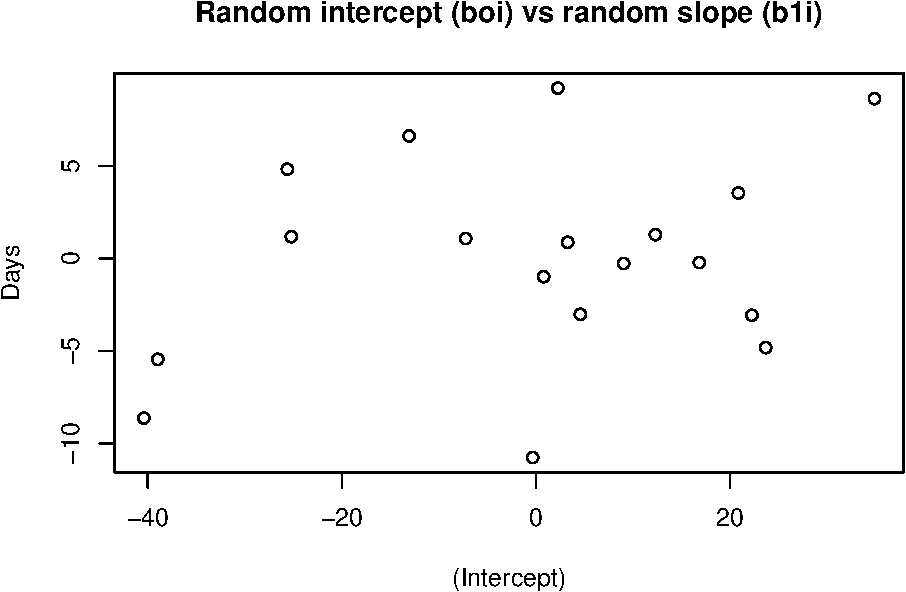
\includegraphics{common_sleep_files/figure-latex/unnamed-chunk-8-1.pdf}
Next, we plot the predicted random effects of the intercept \(b_{0i}\)
compared to the random effects of the slope \(b_{1i}\). These random
effects reflect how the evolution of the ith Subject deviates from the
expected evolution.

\hypertarget{ols-vs-lmm-estimates}{%
\subsubsection{OLS vs LMM estimates}\label{ols-vs-lmm-estimates}}

\begin{center}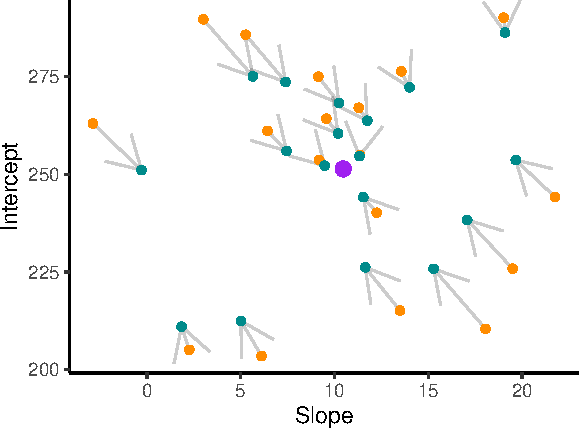
\includegraphics{common_sleep_files/figure-latex/unnamed-chunk-9-1} \end{center}

Having checked the fixed and random effects of the overall linear
regression model, we now compare the original subject-specific
regression model to the multilevel regression model we used for the full
data set. (i.e.~comparing the Ordinary Least Squares (OLS) model to the
Linear Mixed Model (LMM))

Figure A displays the shrinkage effect of the LMM compared to OLS. If we
fit a linear model to each individual subject separately (OLS model)
without taking into account the data of the whole population (orange
dots), intercepts and slopes vary largely. However, if we fit one linear
model to all subjects (LMM, blue dots) the values for intercept and
slope move more closely to the average population intercept and slope
(purple dot).

\hypertarget{conclusion}{%
\subsection{Conclusion}\label{conclusion}}

From our analysis on the effect of sleep deprivation on the reaction
time of long distance truck drivers, we can conclude that there is a
linear relationship between the amount of days of sleep deprivation and
the reaction time. More precisely, as the sleep deprivation proceeds,
the time needed for a driver to respond to a visual stimulus is
increasing by 10.47 ms (sd = 5.92) per day, on average. The reaction
time of people before they were sleep deprived averages 251.41 ms (sd =
24.74).

Several groups of drivers with different conditions of restricted sleep
deprivation or a control group would additionally help us draw a more
concrete conclusion. From the existing literature, mathematical models
predicting alertness from preceding sleep-wake history typically involve
four factors: sleep homeostasis, circadian rhythm, sleep inertia and
neuromodulatory changes. Thus, we can conclude that there is a relation
between reaction time and sleep deprivation, but it is not the only
factor that can fully describe the relationship of sleep deprivation and
the reaction time.

\end{document}
